\begin{frame}
    \frametitle{Integral formulation SCF}
    \begin{columns}
    \begin{column}[b]{0.5\textwidth}

    \centering
    \textbf{Kohn-Sham equations}
    \begin{equation}
        \nonumber
        \left[\hat{T} + \hat{V}\right]\ket{\orbital_i} =\ 
        \epsilon_i \ket{\orbital_i}
    \end{equation}

    \vspace{5mm}

    \textbf{Bound-State Helmholtz operator}
    \begin{equation}
        \nonumber
        2\hat{G}_i  = \left[\hat{T} - \epsilon_i\right]^{-1} 
    \end{equation}

    \vspace{5mm}

    \textbf{Iterative solution}
    \begin{equation}
        \nonumber
        \ket{\orbital_i}^{n+1} =\ -2\Helmholtz{\hat{V}^n\ket{\orbital_i}^n}
    \end{equation}

    \vspace{10mm}
    \end{column}

    \begin{column}[b]{0.5\textwidth}
%    \begin{figure}
%        \includegraphics[scale=0.2, clip, viewport = 100 450 400 720]
%        {figures/methane.pdf}
%        \includegraphics[scale=0.3, clip, viewport = 320 200 520 400]
%        {figures/methaneGrid.pdf}
%    \end{figure}
%    \begin{figure}
%        \includegraphics[scale=0.6, clip, viewport = 50 350 300 540]
%        {figures/convergence.pdf}
%    \end{figure}
    \begin{figure}
	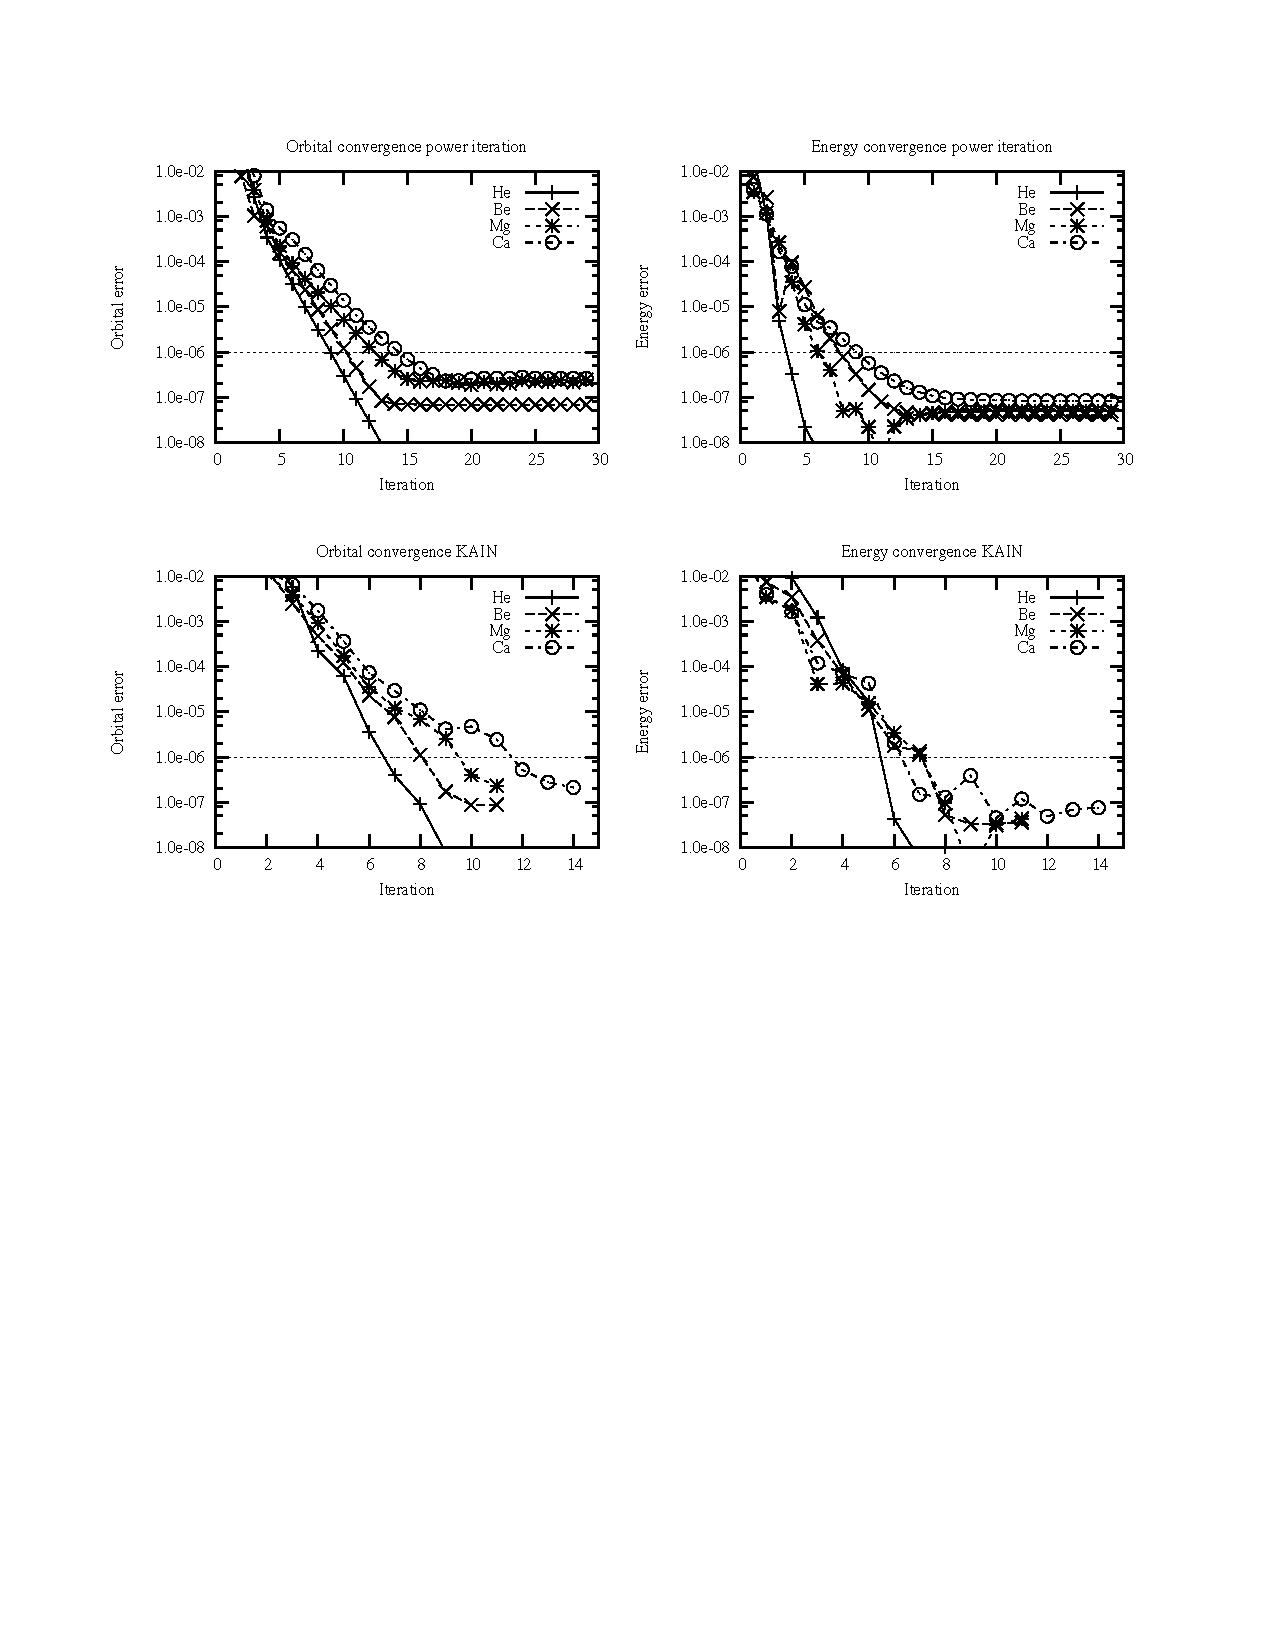
\includegraphics[scale=0.55, clip, viewport = 50 565 300 715]
                {figures/accuracy.pdf}\\
	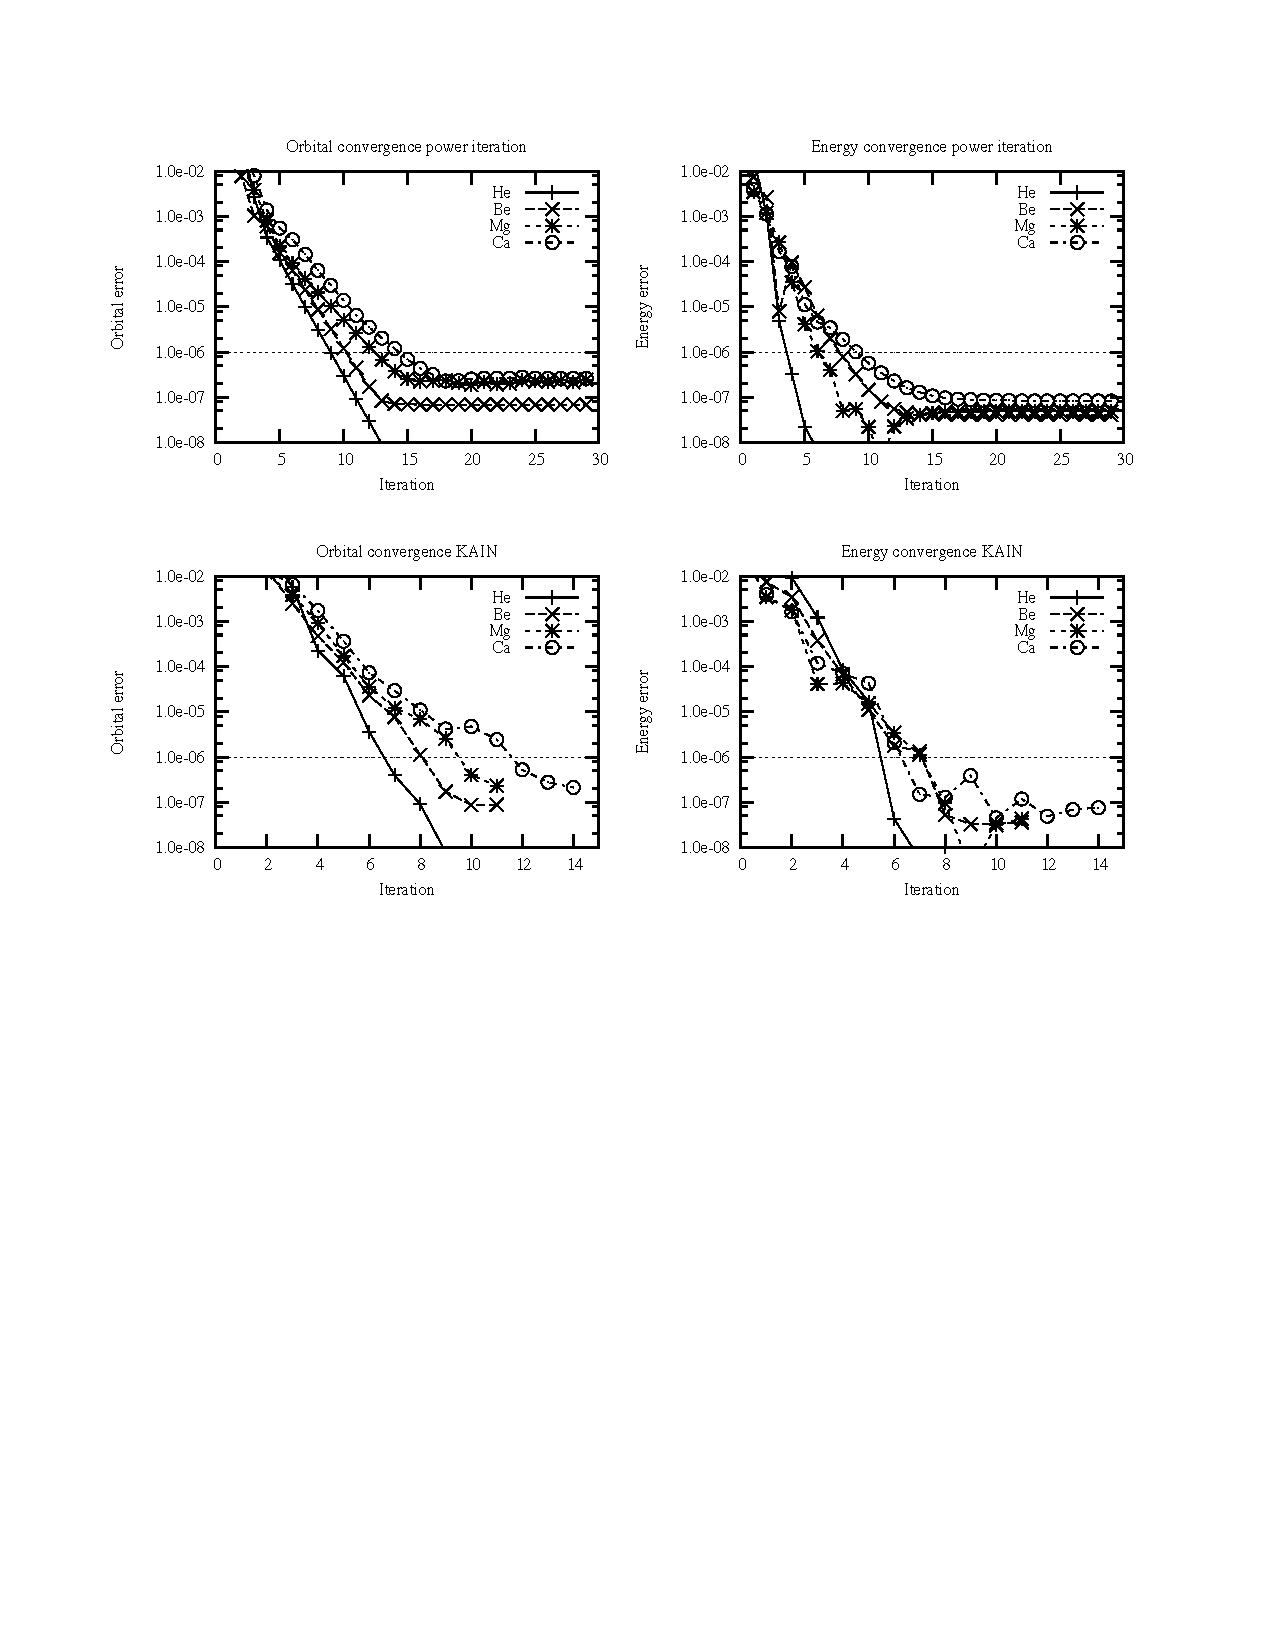
\includegraphics[scale=0.55, clip, viewport = 301 550 551 715]
                {figures/accuracy.pdf}
    \end{figure}

    \end{column}
    \end{columns}

    %\centering
    %\vspace{2mm}
    %\tiny
    %M.H. Kalos, 
    %{\it Phys. Rev.}, 
    %\textbf{128(4)}
    %(1962)\\
    %R.J. Harrison \etal,
    %{\it J. Chem. Phys.}, 
    %\textbf{121}
    %(2004)
\end{frame}

%\begin{frame}
%    \frametitle{Orbital localization}
%    \begin{columns}
%    \begin{column}[b]{0.48\linewidth}
%    \begin{center}
%    \textbf{Canonical}
%    \begin{equation}
%        \nonumber
%        \orbital_i^{n+1} =\ -2\hat{G}_i\Bigg[\hat{V}^n\orbital_i^n\Bigg]
%    \end{equation}
%
%    \vspace{8mm}
%
%    \includegraphics[scale=0.3, clip, viewport = 80 560 600 700]
%        {figures/alkane.pdf}\\
%    \includegraphics[scale=0.3, clip, viewport = 80 560 600 700]
%        {figures/can_orb_1.pdf}\\
%    \includegraphics[scale=0.3, clip, viewport = 80 560 600 700]
%        {figures/can_orb_2.pdf}
%    \end{center}
%    \end{column}
%
%    \begin{column}[b]{0.48\linewidth}
%    \begin{center}
%    \only<2>{
%    \textbf{Localized}
%    \begin{equation}
%        \nonumber
%        \orbital_i^{n+1} =\ -2\Helmholtz{\hat{V}^n\orbital_i^n
%        - \sum_{j\neq i}F^n_{ij}\orbital_j^n}
%    \end{equation}
%    }
%
%    \vspace{8mm}
%
%    %\only<1>{\includegraphics[scale=0.3, clip, viewport = 80 160 600 300]
%        %{figures/loc_orb_1.pdf}\\}
%    %\only<1>{\includegraphics[scale=0.3, clip, viewport = 80 160 600 300]
%        %{figures/loc_orb_2.pdf}\\}
%    %\only<1>{\includegraphics[scale=0.3, clip, viewport = 80 160 600 300]
%        %{figures/loc_orb_3.pdf}}
%    \only<2>{\includegraphics[scale=0.3, clip, viewport = 80 560 600 700]
%        {figures/loc_orb_1.pdf}\\}
%    \only<2>{\includegraphics[scale=0.3, clip, viewport = 80 560 600 700]
%        {figures/loc_orb_2.pdf}\\}
%    \only<2>{\includegraphics[scale=0.3, clip, viewport = 80 560 600 700]
%        {figures/loc_orb_3.pdf}}
%    \end{center}
%    \end{column}
%    \end{columns}
%    \only<1,2>{
%    \vspace{5mm}
%    \centering
%    \tiny
%    S.F. Boys,
%    {\it Rev. Mod. Phys.}, 
%    \textbf{32:296}
%    (1960)\\
%    J.M. Foster, S.F. Boys,
%    {\it Rev. Mod. Phys.}, 
%    \textbf{32:300}
%    (1960)
%    }
%\end{frame}

%\begin{frame}
%    \frametitle{Calculation of Fock matrix}
%    \begin{columns}
%    \begin{column}[b]{0.55\textwidth}
%    \centering
%    We need to calculate the Fock matrix
%    \begin{equation}
%        \nonumber
%        F_{ij} = \langle \orbital_i | \hat{T} + \hat{V} | \orbital_j \rangle
%    \end{equation}
%
%    \vspace{5mm}
%
%    The kinetic part can be calculated using first order \\
%    differential operators
%    \begin{equation}
%        \nonumber
%        T_{ij} =
%        \langle \orbital_i | -\frac{1}{2}\nabla^2 | \orbital_j \rangle = 
%        \frac{1}{2}\langle \nabla \orbital_i | \nabla \orbital_j \rangle 
%    \end{equation}
%
%    \vspace{8mm}
%    \pause
%
%    But we can also compute the \textbf{exact} Fock matrix at a given iteration 
%    without any reference to the kinetic energy operator
%
%    \begin{align}
%        \nonumber
%        F^{n+1}    &= F^n + \Delta F^n\\
%        \nonumber
%        \Delta F^n &= \Delta S_1^nF^{n}+\Delta S_2^n\Lambda^n+\Delta F_{pot}^n\\
%        \nonumber
%        & \\
%        \nonumber
%        (\Delta S_1^n)_{ij} &= \langle \Delta \orbital_i^n | \orbital_j^n \rangle\\
%        \nonumber
%        (\Delta S_2^n)_{ij} &= \langle \orbital_i^{n+1} | \Delta \orbital_j^n \rangle\\
%        \nonumber
%        (\Delta F_{pot}^n)_{ij}
%        &= \langle \orbital_i^{n+1} | \hat{V}^n | \Delta\orbital_j^n \rangle
%        + \langle \orbital_i^{n+1} | \Delta\hat{V}^n | \orbital_j^n \rangle
%    \end{align}
%
%    \vspace{2mm}
%
%    \end{column}
%
%    \begin{column}[b]{0.45\textwidth}
%    \begin{figure}
%	\includegraphics[scale=0.5, clip, viewport = 50 550 300 740]
%                {figures/accuracy.pdf}
%    \end{figure}
%    \begin{figure}
%	\includegraphics[scale=0.5, clip, viewport = 300 550 550 740]
%                {figures/accuracy.pdf}
%    \end{figure}
%
%    \end{column}
%    \end{columns}
%\end{frame}


%\begin{frame}
%    \frametitle{Hydrogen atom}
%    \centering
%    \textbf{Power iteration}
%    \begin{equation}
%	\nonumber
%	\orbital^{n+1} = -2\hat{H}\left[v_{nuc}\orbital^n\right]
%    \end{equation}
%    \ \\
%    \ \\
%    \ \\
%    \begin{columns}
%    \begin{column}{.10\textwidth}
%    \ \\
%    \end{column}
%    \begin{column}{.40\textwidth}
%    \centering
%    \textbf{Orbital update}
%    \begin{equation}
%	\nonumber
%	\Delta\orbital^n = \orbital^{n+1} - \orbital^n
%    \end{equation}
%    \end{column}
%    \begin{column}{.50\textwidth}
%    \centering
%    \textbf{Energy update}
%    \begin{equation}
%	\nonumber
%	\Delta \epsilon^n = \left<\orbital^{n+1}|v_{nuc}|\Delta\orbital^n\right>
%    \end{equation}
%    \end{column}
%    \end{columns}    
%    \begin{center}
%	\includegraphics[scale=0.6, clip, viewport = 50 550 540 730]
%       {figures/convergence.pdf}
%    \end{center}
%\end{frame}

%\begin{frame}
%    \frametitle{Hydrogen atom}
%    \only<1>{\includegraphics[viewport = 50 430 300 640, clip, scale=1.2]
%       {figures/s1Orb_1.pdf}}
%    \only<2>{\includegraphics[viewport = 50 430 300 640, clip, scale=1.2]
%       {figures/s1Orb_2.pdf}}
%    \only<3>{\includegraphics[viewport = 50 430 300 640, clip, scale=1.2]
%       {figures/s1Orb_3.pdf}}
%    \only<4>{\includegraphics[viewport = 50 430 300 640, clip, scale=1.2]
%       {figures/s1Orb_4.pdf}}
%    \only<5>{\includegraphics[viewport = 50 430 300 640, clip, scale=1.2]
%       {figures/s1Orb_5.pdf}}
%    \only<6>{\includegraphics[viewport = 50 430 300 640, clip, scale=1.2]
%       {figures/s1Orb_10.pdf}}
%\end{frame}

%\begin{frame}
%    \frametitle{Many-electron systems}
%    \begin{columns}
%    \begin{column}[b]{0.1\textwidth}
%    \ \\
%    \end{column}
%    \begin{column}[b]{0.4\textwidth}
%    \centering
%    Density
%    \begin{equation}
%	\nonumber
%	\rho^n(\boldsymbol{r}) = \sum_i |\orbital_i^n(\boldsymbol{r})|^2
%    \end{equation}
%    \end{column}
%    \begin{column}[b]{0.4\textwidth}
%    \centering
%    Potentials
%    \begin{equation}   
%	\nonumber
%	\rho^n(\boldsymbol{r}) \rightarrow v_{eff}^n(\boldsymbol{r})
%    \end{equation}
%    \end{column}
%    \begin{column}[b]{0.1\textwidth}
%    \ \\
%    \end{column}
%    \end{columns}
%    \ \\
%    \ \\
%    \begin{columns}
%    \begin{column}[b]{0.1\textwidth}
%    \ \\
%    \end{column}
%    \begin{column}[b]{0.4\textwidth}
%    \centering
%    Power iteration
%    \begin{equation}
%	\nonumber
%	\tilde{\orbital}_i^n = -2\hat{H}\left[v_{eff}^n\orbital_i^n\right]
%    \end{equation}
%    \end{column}
%    \begin{column}[b]{0.4\textwidth}
%    \centering
%    Calculate updates
%    \begin{equation}
%	\nonumber
%	\Delta\orbital^n = \tilde{\orbital}^n - \orbital^n
%    \end{equation}
%    \end{column}
%    \begin{column}[b]{0.1\textwidth}
%    \ \\
%    \end{column}
%    \end{columns}
%    \ \\
%    \ \\
%    \pause
%    \only<1,2>{
%    \centering
%    \ \\
%    \textbf{Complicating issues}
%    \ \\
%    \begin{columns}
%    \begin{column}[b]{0.25\textwidth}
%    \ \\
%    \end{column}
%    \begin{column}[b]{0.75\textwidth}
%    \begin{itemize}
%	\item	Straightforward iteration will bring all\\ 
%		orbitals to the lowest energy eigenfunction
%	\item	Orthonormality must be imposed
%	\item	Achieved by diagonalizing the Fock matrix 
%    \end{itemize}
%    \end{column}
%    \end{columns}
%    \begin{equation}
%        \nonumber
%        F_{ij} = \left<\orbital_i|\hat{T} + v_{eff}|\orbital_j\right>
%    \end{equation}
%    \ \\
%    \ \\
%    \ \\
%    \ \\
%    }
%    \only<3,4,5>{
%    \centering
%    Compute Fock matrix update
%    \begin{equation}
%	\nonumber
%	\Delta F_{ij}^n = \left<\tilde{\orbital}_i^n|v_{eff}^n |\Delta\orbital_j^n\right>
%			    + \left<\tilde{\orbital}_i^n|\Delta
%			    v_{eff}^n|\orbital_j^n\right>
%    \end{equation}
%    \ \\
%    \ \\
%    \ \\
%    \pause
%    \pause
%    \begin{columns}
%    \begin{column}[b]{0.1\textwidth}
%    \ \\
%    \end{column}
%    \begin{column}[b]{0.4\textwidth}
%    \centering
%    Diagonalize matrix
%    \begin{equation}
%	\nonumber
%	F^{n+1} = M^{-1}\tilde{F}^nM
%    \end{equation}
%    \end{column}
%    \begin{column}[b]{0.4\textwidth}
%    \centering
%    Rotate orbitals
%    \begin{equation}
%	\nonumber
%	\orbital_i^{n+1} = \sum_jM^{-1}_{ij}\tilde{\orbital}_j^n
%    \end{equation}
%    \end{column}
%    \begin{column}[b]{0.1\textwidth}
%    \ \\
%    \end{column}
%    \end{columns}
%    \ \\
%    \ \\
%    \pause
%    Compute iterative subspace acceleration (KAIN or DIIS)\\
%    \ \\
%    Orthonormalize\\
%    \ \\
%    }
%\end{frame}

%\begin{frame}
%\frametitle{Accurate calculations}
%\centering
%\begin{table}
%    \centering
%    \begin{tabular}{lr@{.}lr@{.}l}
%    \multicolumn{5}{c}{\textbf{LDA energy of Argon (a.u.)}}\\
%    \hline
%    \hline
%                        &\multicolumn{4}{c}{}   \\
%    &\multicolumn{2}{c}{HOMO}
%    &\multicolumn{2}{c}{Total}\\
%                        &\multicolumn{4}{c}{}   \\
%    MW $\epsilon=10^{-3}$  &-0&387692&-525&966790  \\
%    MW $\epsilon=10^{-5}$  &-0&382348&-525&946109  \\
%    MW $\epsilon=10^{-7}$  &-0&382330&-525&946196  \\
%                        &\multicolumn{4}{c}{}   \\
%    NIST                &-0&382330&-525&946195  \\
%                        &\multicolumn{4}{c}{}   \\
%    aug-cc-pV6Z		&-0&382323&-525&944181  \\
%%    aug-cc-pV5Z		&-0&382388&-525&942021  \\
%    aug-cc-pVQZ		&-0&382463&-525&938021  \\
%%    aug-cc-pVTZ	        &-0&382838&-525&933682  \\
%    aug-cc-pVDZ		&-0&382143&-525&915702  \\
%                        &\multicolumn{4}{c}{}   \\
%    \hline
%    \hline
%    \end{tabular}
%\end{table}
%
%\vspace{1mm}
%
%\it{NIST: National Institute of Standards and Technology (Basis set limit)}\\
%\it{GTO calculations using Dalton}
%
%\vspace{5mm}
%
%\begin{itemize}
%    \item   We are able to attain \textbf{considerably higher} accuracy than 
%            high-quality Gaussian basis sets
%    \item   Energies are not variational, but \textbf{basis set limit} within 
%            the requested precision
%    \item   Calculations are still more expensive than conventional methods
%\end{itemize}
%
%\end{frame}


%\begin{frame}
%    \frametitle{Accurate calculations}
%    \centering
%    Replacing the exchange-correlation potential $v_{xc}$ with the exact exchange operator
%    \begin{equation}
%	\nonumber
%	\hat{K}\orbital_i(\boldsymbol{r}) = \sum_j \orbital_j(\boldsymbol{r}) 
%	\int P(\boldsymbol{r}-\boldsymbol{r}')
%	\left[\orbital_i(\boldsymbol{r}')\orbital_j(\boldsymbol{r}')\right] d\boldsymbol{r}'
%    \end{equation}
%    gives the Hartree-Fock equations, which can be solved by the same iterative methods
%    \ \\
%    \ \\
%\begin{table}
%\tiny
%\begin{tabular}{cllll}
%\hline   
%\hline
%\multicolumn{5}{c}{Total Hartree-Fock energies in atomic units (Hartree)}\\
%&\multicolumn{1}{c}{H$_2$O}
%&\multicolumn{1}{c}{H$_2$O$_2$}
%&\multicolumn{1}{c}{CO}
%&\multicolumn{1}{c}{CO$_2$}\\
%\hline 
%            		    &               &               &               &               \\
%MRChem $\epsilon=10^{-5}$   & -76.067611455 & -150.85253297 & -112.79087294 & -187.72538886 \\
%MRChem $\epsilon=10^{-6}$   & -76.067556696 & -150.85249254 & -112.79069389 & -187.72541991 \\
%MRChem $\epsilon=10^{-7}$   & -76.067535613 & -150.85246986 & -112.79081263 & -187.72538522 \\
%MRChem $\epsilon=10^{-8}$   & -76.067535431 & -150.85247037 & -112.79081269 & -187.72538560 \\
%            		    &               &               &               &               \\
%Est. HF limit		    & -76.0675      & -150.8525     & -112.7908     & -187.7254     \\
%            		    &               &               &               &               \\
%aug-cc-pCV5Z		    & -76.067379371 & -150.85218780 & -112.79063514 & -187.72508317 \\
%aug-cc-pCVQZ		    & -76.066140457 & -150.84985235 & -112.78919290 & -187.72260431 \\
%            		    &               &               &               &               \\
%\hline   
%\hline   
%\end{tabular}
%\end{table}
%\ \\
%\ \\
%\ \\
%\begin{itemize}
%    \item   We are able to attain \textbf{considerably higher} accuracy than high-quality 
%	    Gaussian basis sets
%    \item   Energies are not variational, but \textbf{basis set limit} within the requested 
%	    precision
%    \item   Calculations are still more expensive than conventional methods
%\end{itemize}
%\end{frame}

%\begin{frame}
%\frametitle{Ground state energy}
%
%\centering
%\textbf{Methyloxirane molecule}
%\hspace{30mm}
%\textbf{Adaptive grid}
%\begin{minipage}{0.5\textwidth}
%\centering
%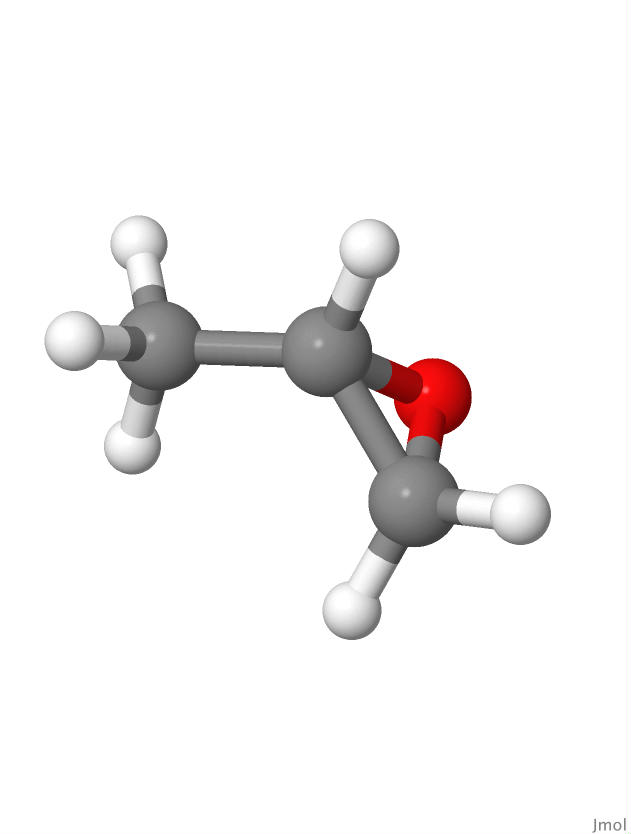
\includegraphics[scale=0.15, viewport = 0 180 550 650, clip]{figures/methyloxirane_white.jpg}
%\end{minipage}%
%\begin{minipage}{0.5\textwidth}
%\centering
%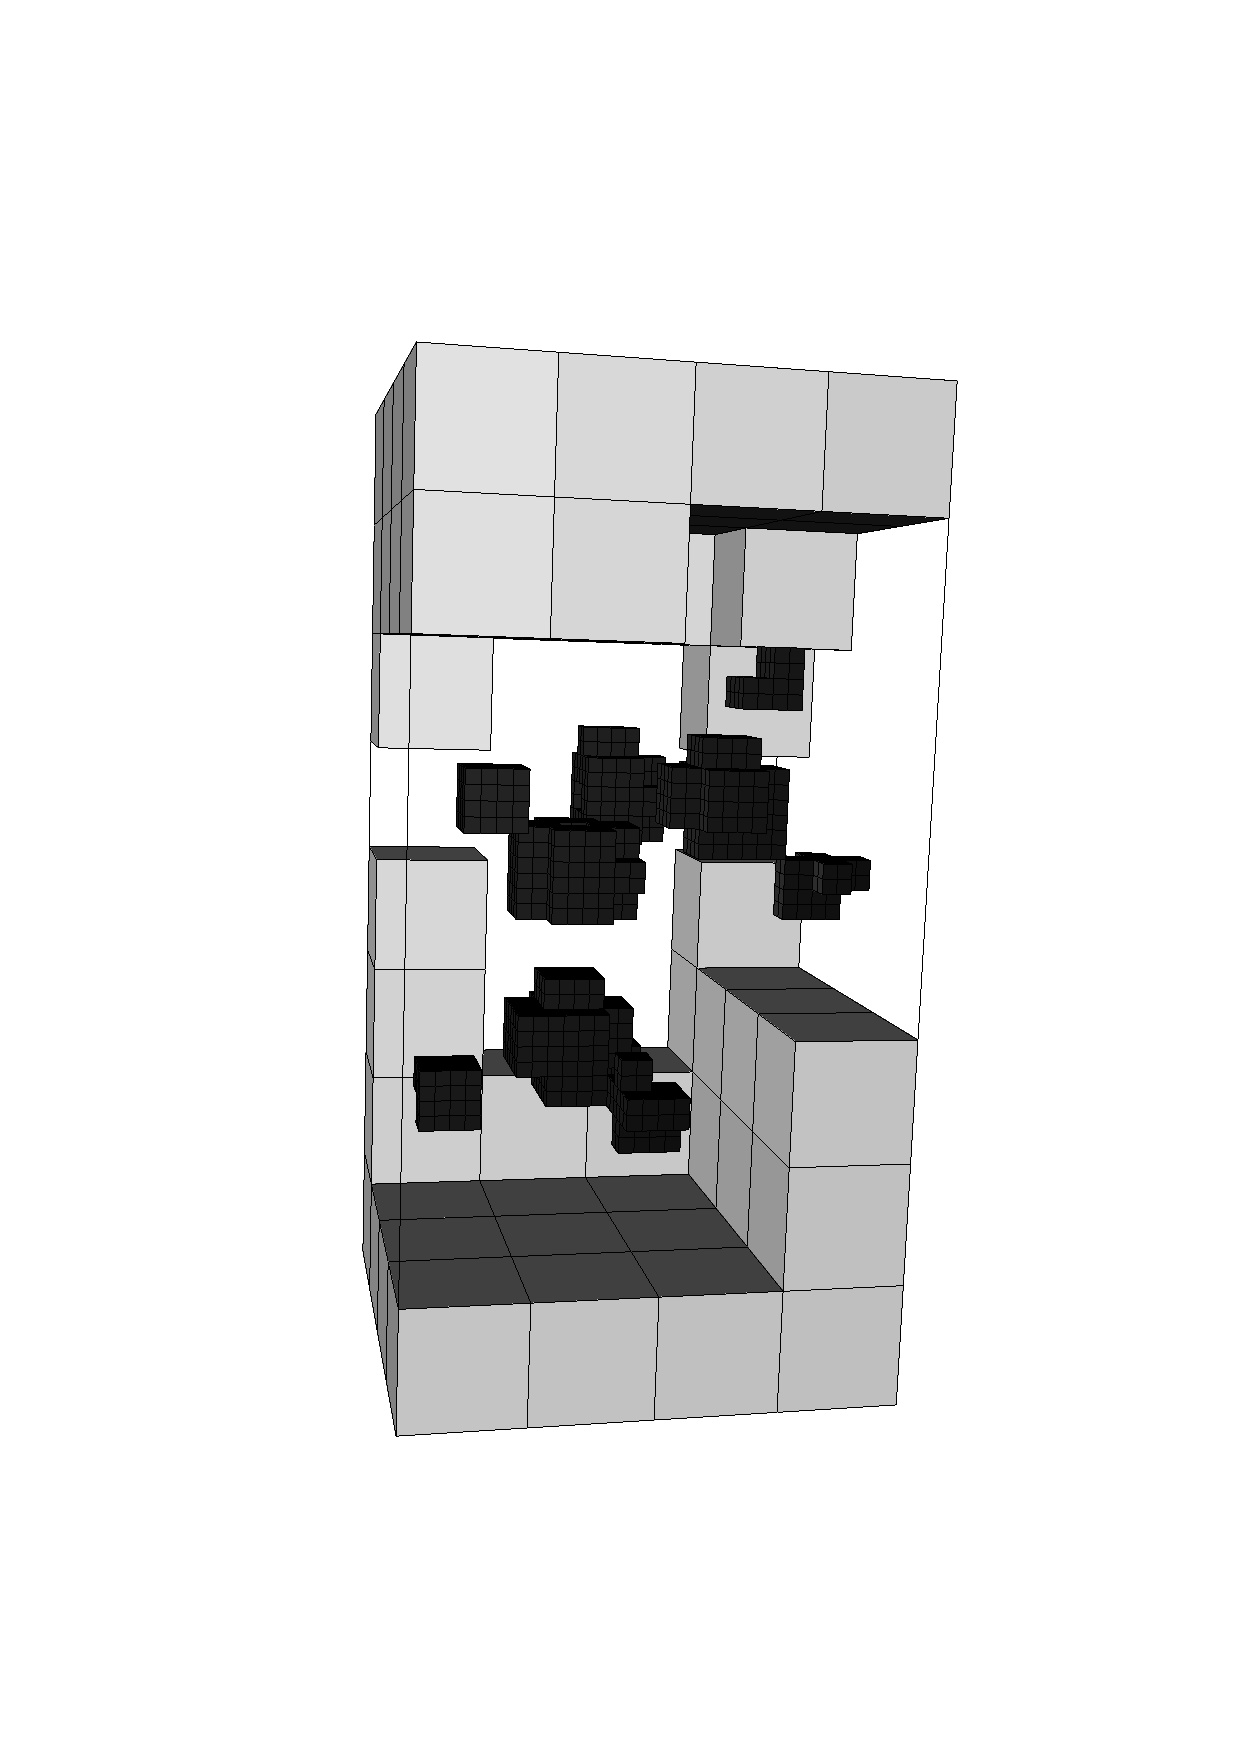
\includegraphics[angle=-90, scale=0.25, viewport = 170 150 470 700, clip]{figures/methyloxirane_grid.pdf}
%\end{minipage}
%
%\vspace{5mm}
%
%\begin{table}
%    \centering
%    \begin{tabular}{r|cr|cr}
%    \multicolumn{5}{c}{\textbf{Total energy (a.u.)}}\\
%    \hline               
%    \hline               
%                     &               &               &               &               \\
%                     &Hartree-Fock   &Time           &LDA            &Time           \\
%    \hspace{20mm}\   &\hspace{20mm}\ &\hspace{05mm}\ &\hspace{20mm}\ &\hspace{05mm}\ \\
%    MRChem $10^{-2}$ & -192.0425     &  30m          & -191.5975     &   2m          \\
%    MRChem $10^{-3}$ & -192.0002     &   1h          & -191.5622     &   5m          \\
%    MRChem $10^{-4}$ & -192.0000     &   3h          & -191.5619     &  10m          \\
%                     &               &               &               &               \\
%    aug-cc-pVQZ      & -191.9968     &  30m          & -191.5563     &  30m          \\
%        cc-pVQZ      & -191.9960     &  10m          & -191.5549     &  10m          \\
%    aug-cc-pVDZ      & -191.9357     &  $<$1m        & -191.4817     &  $<$1m        \\
%        cc-pVDZ      & -191.9232     &  $\ll$1m      & -191.4622     &  $\ll$1m      \\
%                     &               &               &               &               \\
%    \hline
%    \hline
%    \end{tabular}
%\end{table}
%
%\centering
%\it{Wall time given on 16 CPUs}\\
%\it{GTO calculations using Dalton}
%
%\end{frame}


